% !TeX document-id = {a9da8c09-8ca2-42d8-97aa-816e53d9f143}
% !TeX TXS-program:compile = txs:///latexmk/{}[-xelatex -synctex=1 -interaction=nonstopmode -silent %.tex]

\documentclass[hideanswer=true,
enfont=empty,	%在settings.tex里由zhfont指定
zhfont=empty,	%在settings.tex里由zhfont指定
mathfont=newtxmath,
]{cmcthesis}

\cmcthesissetup{% key = value 设置处
	%
}

\let\leq\leqslant\let\geq\geqslant
\def\sgn{\mathop{\rm sgn}}
\everymath{\displaystyle}

\newcommand{\ee}{\mathrm e}
\newcommand{\dd}{\,\mathrm{d}}
\newcommand{\textop}[1]{\relax\ifmmode\mathop{\text{#1}}\else\text{#1}\fi}
%%%%%%定义两个列格式,数学与非数学模式
\newcolumntype{Y}{>{\centering\arraybackslash$}X<{$}}
\newcolumntype{Z}{>{\centering\arraybackslash}X}
\newcolumntype{L}{>{\raggedright\arraybackslash}X}
\newcolumntype{R}{>{\raggedleft\arraybackslash}X}
%定义绝对值
\newcommand\abs[1]{\left| #1 \right|}
\makeatletter
\newcommand{\rmnum}[1]{\romannumeral #1}
\newcommand{\Rmnum}[1]{\expandafter\@slowromancap\romannumeral #1@}
\makeatother

%%%%%%%%%%%%%%%%%%%%%%%%%%%%%%%%%%%%%%%%%%%%%%

\newcommand{\chaoda}{\fontsize{55pt}{\baselineskip}\selectfont}
\newcommand{\chuhao}{\fontsize{42pt}{\baselineskip}\selectfont}     % 字号设置
\newcommand{\xiaochuhao}{\fontsize{36pt}{\baselineskip}\selectfont} % 字号设置
\newcommand{\yihao}{\fontsize{28pt}{\baselineskip}\selectfont}      % 字号设置
\newcommand{\erhao}{\fontsize{21pt}{\baselineskip}\selectfont}      % 字号设置
\newcommand{\xiaoerhao}{\fontsize{18pt}{\baselineskip}\selectfont}  % 字号设置
\newcommand{\sanhao}{\fontsize{15.75pt}{\baselineskip}\selectfont}  % 字号设置
\newcommand{\xiaosanhao}{\fontsize{15pt}{\baselineskip}\selectfont} % 字号设置
\newcommand{\sihao}{\fontsize{14pt}{\baselineskip}\selectfont}      % 字号设置
\newcommand{\xiaosihao}{\fontsize{12pt}{14pt}\selectfont}           % 字号设置
\newcommand{\wuhao}{\fontsize{10.5pt}{12.6pt}\selectfont}           % 字号设置
\newcommand{\xiaowuhao}{\fontsize{9pt}{11pt}{\baselineskip}\selectfont}   % 字号设置
\newcommand{\liuhao}{\fontsize{7.875pt}{\baselineskip}\selectfont}  % 字号设置
\newcommand{\qihao}{\fontsize{5.25pt}{\baselineskip}\selectfont}    % 字号设置

\everymath{\displaystyle}
\usepackage[thmmarks,amsmath]{ntheorem}
\theoremstyle{nonumberplain}
\theoremheaderfont{\bfseries}
\theorembodyfont{\normalfont}
{
	\theoremstyle{nonumberplain}%不带标号
	\theoremheaderfont{\bfseries}%证明题头加粗
	\theorembodyfont{\normalfont}
	%	\theorembodyfont{\songti}%楷书字体
	\theoremsymbol{\mbox{$\Box$}}%结束以后自动画出一个小方块
	\newtheorem{solution}{解.}%名字叫做"solution",会在题头自动写上证明
}
{
	\theoremstyle{nonumberplain}%不带标号
	\theoremheaderfont{\bfseries}%证明题头加粗
	\theorembodyfont{\normalfont}
	%	\theorembodyfont{\songti}%楷书字体
	\theoremsymbol{\mbox{$\blacksquare$}}%结束以后自动画出一个小黑色方块
	%	\theoremsymbol{\mbox{$\Box$}}%结束以后自动画出一个小方块
	\newtheorem{proof}{证明.}%名字叫做"proof",会在题头自动写上证明
}


\begin{document}

	\cmcthesistitle{
		name    = 嘉善县火种计划试点学校信息技术阶段测试 ,
		subname = Python 试题,
		date    =  2021年6月 \thinspace , % 9:00 - 11:30  ,
%		author  = (火种计划命题组)  ,
		motto   = 技术支持:红码科技,
	}
	
\addvspace{1\bigskipamount}

%\verb|hideanswer=false,true| 两个选项可以选择一个。它决定了 \verb|answer| 环境里面的内容是否显示,以及开头的说明和页脚的内容。

\makepart{填空题}{共5小题,每题4分,共计20分}

\begin{problem}
	已知a = 1, b = 2, 表达式 a == b or 3 的值为 \fillin{ 3 }.
\end{problem}

\begin{problem}
	表达式 'ab' in 'acbed' 的值为 \fillin{ False }.
\end{problem}

\begin{problem}
	在循环语句中, \fillin{ break } 语句的作用是提前结束循环.
\end{problem}

\begin{problem}
	令 x = [1, 2, 3, 2, 3], 执行x.pop(3)后, x的值为 \fillin{ [1, 2, 3, 3] }.
\end{problem}

\begin{problem}
	已知a = 3, b = 9, 执行a, b = b, a后, 表达式a / b 的值是 \fillin{ 3.0 }.
\end{problem}
\begin{answer}
	\textbf{注意: 第5题写整数3不给分.}
\end{answer}

\makepart{单项选择题}{共15小题,每题4分,共计60分}

\begin{problem}
	下列关于分支和循环结构的描述中,错误的是  \pickout{ D }
	\options
	{for循环可以用while循环改写}
	{While循环只能用来实现无限循环}
	{保留字break可以终止一个循环}
	{continue可以跳过本次循环后续代码的执行, 并继续执行下一次循环}	
\end{problem}

\begin{problem}
	下列Turtle库中画笔属性说法\uline{不正确}的是:  \pickout{ D }
	\options
	{\texttt{turtle.pensize()} :设置画笔的宽度}	%\verb|text| 不能用
	{\texttt{turtle.pencolor()} :设置画笔的颜色}
	{\texttt{turtle.speed()} :设置画笔移动速度}
	{\texttt{turtle.distance()} :设置画笔移动距离}
\end{problem}

\begin{problem}
	courses = ["C++", "Java", "Python", "HTML"],运行courses.pop()后, course会变成  \pickout{ B }
	\options
	{["Java", "Python", "HTML"]}
	{["C++", "Java", "Python"]}
	{["C++", "Python", "HTML"]}
	{[]}
\end{problem}

\begin{problem}
	假设\texttt{a = 8}, \texttt{b = 2}, 那么在python中计算\texttt{a / b * b}的结果是          \pickout{  C  }
	\options
	{\texttt{8}          }
	{\texttt{2}                     }
	{\texttt{8.0}                     }
	{\texttt{2.0}                     }
\end{problem}

\begin{problem}
	这段代码的运行结果是          \pickout{  B  }
	\begin{lstlisting}[style=tex, language=python]
		poem = "明日复明日"
		for i in poem:
		    if i == "明":
		        continue
		print(i)
	\end{lstlisting}

	\options
	{ 明复明       }
	{ 日复日                     }
	{ 明明                     }
	{ 明日复明日           }
\end{problem}

\begin{problem}
	如果\texttt{a = 20.0},\texttt{b = 20}, 那么\texttt{print(b == a)}运算的结果是          \pickout{  A  }
	\options
	{\texttt{True}                     }
	{\texttt{False}                     }
	{\texttt{20}                     }
	{\texttt{20.0}                     }

\end{problem}

\begin{problem}
	将3、5、7三个数不重复的排列为三位数,有几种排列?         \pickout{  B  }
	\options
	{\texttt{}         3            }
	{\texttt{}        6             }
	{\texttt{}         9            }
	{\texttt{}          2           }
\end{problem}

\begin{problem}
	执行下面程序,结果是          \pickout{  D  }
	\begin{lstlisting}[style=tex, language=python]
		i = 1
		while i <= 10:
		    if i % 2:
				print(i)
			i += 1
	\end{lstlisting}
	
	\options
	{ 1 3 5 7       }
	{ 2 4 6 8 10                  }
	{ 2 4 6 8                      }
	{ 1 3 5 7 9        }
\end{problem}

\begin{problem}
	a = "3", print(a * 2)的结果是          \pickout{  B  }
	\options
	{       6             }
	{         "33"           }
	{           "6"         }
	{         报错           }
\end{problem}

\begin{problem}
	下列程序哪个是画一个三角形?          \pickout{ A   }
	
	
	\options
	{\fbox[l]{\shortstack[l]{turtle.forward(100) \\ turtle.left(120)	\\ 	turtle.forward(100)\\ turtle.right(60) \\ turtle.backward(100)}}}
	{\fbox[l]{\shortstack[l]{turtle.forward(100)
\\ turtle.left(60)
\\ turtle.forward(100)
\\ turtle.right(60)
\\ turtle.backward(100) }}}
	{\fbox[l]{\shortstack[l]{turtle.forward(100)
\\ turtle.left(120)
\\ turtle.forward(100)
\\ turtle.right(60)
\\ turtle.forward(100) }}}
	{\fbox[l]{\shortstack[l]{turtle.forward(100)
\\ turtle.left(120)
\\ turtle.forward(100) \\ turtle.right(120)
\\ turtle.forward(100)
}}}
		

\end{problem}


%	\centering{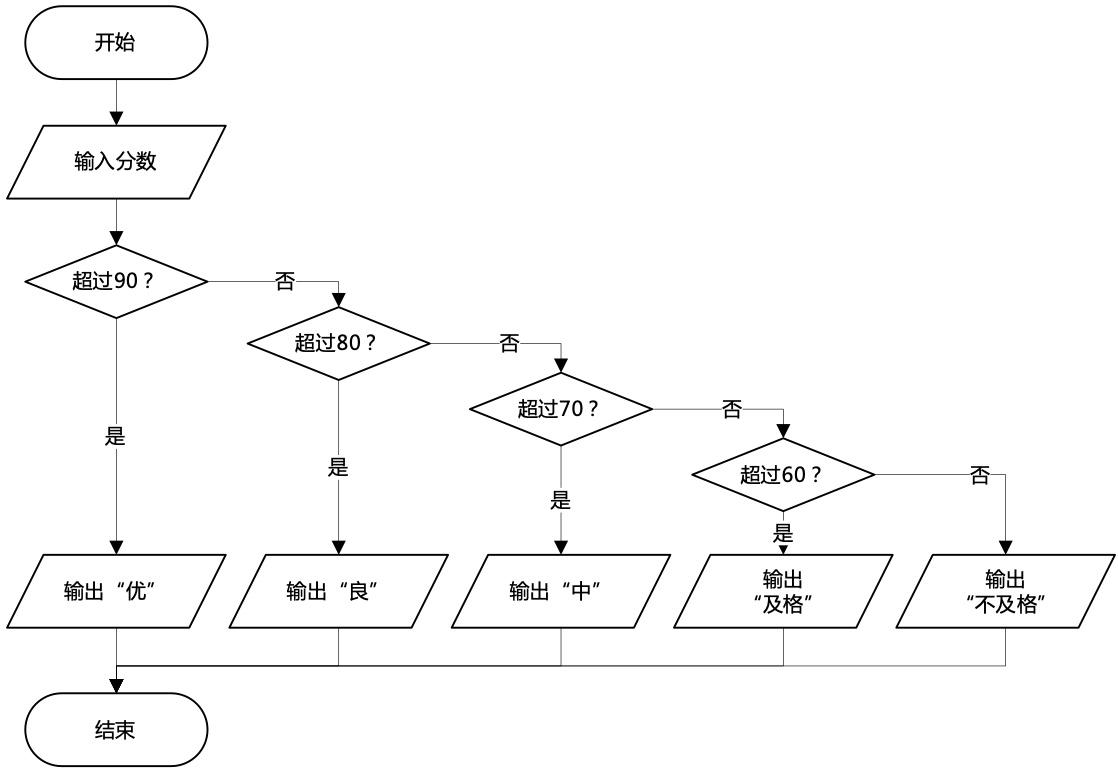
\includegraphics[width=0.5\textwidth]{fig/score}}

\begin{problem}
	关于以下代码的说法正确的是         \pickout{  B  }
	\begin{lstlisting}[style=tex, language=python]
		t = int(input('边数','几边形:')) 
		turtle.circle(50, steps=t)
		turtle.done() 

	\end{lstlisting}

	\options
	{   circle是画圆的代码,因此该程序运行后的图案一定是圆
}
	{  运行该程序后,需要用户自己输入边数,确定画 “几边形”
}
	{  变量t没有给出具体的数值,因此该程序运行有错误
 }
	{  该程序运行后,会画出50个圆                  }
\end{problem}

\begin{problem}
	对于元组里面的元素,可以执行的操作有         \pickout{  C  }
	\options
	{ 添加 
}
	{  修改
}
	{ 查询}
	{  删除  }
\end{problem}

\begin{problem}
	这段代码的运行结果是          \pickout{  A  }
		\begin{lstlisting}[style=tex, language=python]
		t1 = (1, 2, 3, 4, 5, 6, 7)
		t2 = ("a", "b", "c", "d", "e", "f")
		a1 = t1[2:]
		a2 = t2[2:5]
		s = a1 + a2
		print(s) 
	\end{lstlisting}

	\options
	{ (3, 4, 5, 6, 7, 'c', 'd', 'e') }
	{ (4, 5, 6, 7, 'b','c', 'd', 'e')                  }
	{  (3, 4, 5, 6, 7, 'a', b', 'c')                  }
	{ (1,2,3, 4, 5, 'c', 'd', 'e')                   }
\end{problem}

\begin{problem}
	 xiaoming = ["富强", "民主", "文明"], 运行下方代码后会输出          \pickout{  C  }
	\begin{lstlisting}[style=tex, language=python]
		if not ("和谐" in xiaoming):
		    xiaoming.append("和谐")
		print(xiaoming[1] + xiaoming[-1]) 
	\end{lstlisting}
	
	\options
	{ 富强和谐 }
	{ 民主文明                  }
	{  民主和谐                  }
	{ 报错                   }
\end{problem}

\begin{problem}
	字典有键(key)和值(value),以下关于键和值的表述中, \uline{正确}的是         \pickout{  B  }	
	\options
	{ 键(key)和值(value)都是可以重复的 }
	{ 键(key)不可以重复, 值(value)可以重复                }
	{ 键(key)可以重复, 值(value)不可以重复                }
	{ 键(key)和值(value)都是不可以重复的                   }
\end{problem}


\makepart{程序题}{共2题,每题10分,共计20分}

\begin{problem}
	\textbf{程序填空:{\kaishu{(本题共3小题,前两题每题3分,第3小题4分, 共10分)}}} \\
	大聪明在学习了有关质数的课程后, 写了个python程序, 想要输出100以内的所有质数, 但是有几个关键的地方有点卡住了, 你这么热心, 来帮帮他吧! 请仔细阅读下列程序, 并回答问题:
	
\begin{lstlisting}[style=tex, language=python]
	n = 2
	while n <= 100:
	    is_prime = True
	    i = ①_________           
	    while i < n:
	        if ②_________ == 0:
	            is_prime = False
	            break
	        i += 1
	    if is_prime:
	        print(n)
	    ③_________
\end{lstlisting}
	\begin{enumerate}[label=\arabic*), parsep=0ex,itemsep=0ex,leftmargin=2em, topsep=0ex]
		\item 为了得到全部正确的结果, ①处应该填写 \fillin{  2  }
		\item 怎样才能判断一个数是不是素数呢? ②处应该填写 \fillin{ n \% i }
		\item 大聪明写完之后似乎忘记了一些东西, 死活找不出来, 帮他把③处补上吧 \fillin{n += 1}
\end{enumerate}
\end{problem}

\begin{answer}
	\textbf{参考说明:}\\
	本题考查循环和分支结构的综合运用, 初始值, 如何判断整除, 以及如何避免死循环, 是需要掌握的知识点.
	 
	第1题比较简单, 注意不能是1或者3.
	
	第2题判断整除是判断余数是否为零, 需要注意区分比较运算符==和赋值运算符=, 以及不能写成整除符号//.
	
	第3题因为是从2开始遍历的, 所以不能填写 n += 2.
\end{answer}

\begin{problem}
	\textbf{根据描述编写程序求解问题.{\kaishu{(本题10分)}}}
	
	已知3个同学3小时可以打扫完3个房间, 那么n个同学t个小时可以\underline{打扫完}几个房间? 根据上述情况, 在下方横线上编写程序输出结果.

	输入: 两个整数n和t, 需使用输入\\
	输出: 打扫完的房间数r, 整数
	
	\begin{lstlisting}[style=tex, language=python]
	_____________________________________________________________
	_____________________________________________________________
	_____________________________________________________________
	_____________________________________________________________
	_____________________________________________________________
	_____________________________________________________________
	_____________________________________________________________
	_____________________________________________________________
	_____________________________________________________________
	_____________________________________________________________
	_____________________________________________________________
	_____________________________________________________________
	_____________________________________________________________
	_____________________________________________________________
	_____________________________________________________________
	_____________________________________________________________
	\end{lstlisting}
\end{problem}

\begin{answer}
	\textbf{参考说明:}\\
	本题相对简单, 主要考察输入输出, 以及数据类型及转化.
	
	参考代码:
	\begin{lstlisting}[style=tex, language=python]
    n = int(input())  # input()和int()各2分, 共4分, input()括号里有没有提示字符串都可以给分
    t = int(input())  # 如果两条合并到一起赋值而且正确, 可以一起给4分
    r = n * t // 3    # //运算符和计算正确性各2分, 共4分, 用int()转换也可以给分
    print(r)          # 输出结果2分. 另外如果上述代码缩进有误, 每行扣2分
	\end{lstlisting}


\end{answer}

\end{document}